\documentclass[10pt]{beamer}

\mode<presentation>
{
  \usetheme[height=1.25cm]{Madrid}
  \setbeamertemplate{navigation symbols}{}
  \setbeamercolor{alerted text}{fg=illini}
}
\usebackgroundtemplate{
\includegraphics[width=\paperwidth,height=\paperheight]{uc-background}}

\usepackage[english]{babel}
\usepackage{epsfig,subfigure,bm}
\usepackage{multimedia}
\usepackage{psfrag}
\usepackage{animate}

%%%%%% Begin of my macros and options

\setbeamertemplate{section in toc shaded}[default][55]
\setbeamertemplate{subsection in toc shaded}[default][55]
\setbeamercolor{block title}{fg=white,bg=illini}
\setbeamercolor{block body}{fg=black,bg=mygrey}

\setbeamercolor{emphprimary}{fg=CBlue}
\setbeamercolor{emphsecondary}{fg=illini}
\setbeamercolor{emphtertiary}{fg=mygreen}
\definecolor{darkForestGreen}{rgb}{.1,1,.1}
\definecolor{veryLightGray}{rgb}{.9,.9,.9}
\definecolor{greenApple}{rgb}{.3,.9,.3}

\setbeamercolor{frametitle}{bg=CBlue}   
\setbeamercolor{title}{bg=CBlue}

\usepackage{amsmath,amssymb,amsxtra,amsthm}
\usepackage{algorithm,algorithmic}
\usepackage{natbib}
\usepackage{bibentry}
\usepackage{xspace}
\usepackage{changepage}

\pdfmapfile{+sansmathaccent.map}

\definecolor{myblue}{rgb}{.2,.2,.7}
\definecolor{myred}{rgb}{.7,.2,.2}
\definecolor{mygreen}{rgb}{.2,.7,.2}
\definecolor{mygrey}{rgb}{0.9,0.9,0.9}
\definecolor{CBlue}{cmyk}{1,0.25,0,0}
\definecolor{illini}{rgb}{0.98,0.4,0.05}
\definecolor{black}{cmyk}{0,0,0,1}

\newcommand{\myemph}[1]{{\usebeamercolor[fg]{emphprimary}
    \textbf{#1}}}
\newcommand{\myemphalt}[1]{{\usebeamercolor[fg]{emphsecondary}
    \textbf{#1}}}

\graphicspath{{figs/}}

\title[Math for Robotics] % (optional, use only with long paper titles)
{CSE276C - Polynomial Interpolation and Approximation}

\author[H.~I. Christensen] % (optional, use only with lots of authors)
{Henrik I.~Christensen}
% - Give the names in the same order as the appear in the paper.  -
% Use the \inst{?} command only if the authors have different
% affiliation.

\AtBeginSection[]
{
   \begin{frame}
       \frametitle{Outline}
       \tableofcontents[currentsection]
   \end{frame}
}

\institute[UCSD] % (optional, but mostly needed)
{
  \begin{minipage}[c]{.2\textwidth}
    
\includegraphics[width=.65\linewidth]{ucsealnew}%
  \end{minipage}%
  \begin{minipage}[c]{.6\textwidth}
    \small
%%    \begin{center}
      Computer Science and Engineering\\
      University of California, San Diego\\
      \myemph{\url{http://cri.ucsd.edu}}\\          
%%    \end{center}

  \end{minipage}
%%  \vspace*{1ex}
}
%% - Use the \inst command only if there are several affiliations.
%% - Keep it simple, no one is interested in your street address.

\bigskip

\date[Oct 2021]% (optional, should be abbreviation of conference name)
{\small%
  October 2021}

\begin{document}
  
\nobibliography{/Users/hic/Dropbox/bibliography/bib-file}
\bibliographystyle{plain}


\begin{frame}[plain]
  \titlepage
\end{frame}


\section{Introduction}

\begin{frame}
  \frametitle{Introduction}
  \begin{itemize}
  \item Last time we spoke about direct use of data point / simple models
  \item What if we want an explicit functional approximation to data? 
  \item Approximating a function/data by a class of simpler functions
  \item Two main motivations
    \begin{enumerate}
    \item Decomposition of a complicated function into constituent simpler functions to simplify further work
    \item Recover a function from partial or noisy information
    \end{enumerate}
  \item Applications:
    \begin{enumerate}
    \item Signal compression / reconstruction (Fourier would be an example)
    \item Data fitting (line, plane, manifold, ...)
    \item Recovery of a model say CAD recovery
    \end{enumerate}
  \end{itemize}
\end{frame}

\begin{frame}
  \frametitle{Material}
  \begin{itemize}
  \item Numerical Recipes: Chapter 3.4-3.5
  \item Numerical Renaissance: Chapter 5
  \end{itemize}
\end{frame}

\section{Uniform approximation}

\begin{frame}
  \frametitle{Uniform approximation by polynomials}
  \begin{itemize}
  \item Looking at polynomial again
  \item What is the best uniform approximation?
  \item Given a function f: $[a,b] \rightarrow R$ and a polynomial p we can measure the error by the $L_{\infty}$ norm, i.e.,
    \[
      ||f-p||_{\infty} = \max_{a<x<b} | f(x) - p(x) |
    \]
  \item A good approximation is one where the norm is small
  \item Remember Weierstrass' theorem.
  \end{itemize}
\end{frame}

\begin{frame}
  \frametitle{Polynomial approximation}
  \begin{itemize}
  \item Lets restrict the degree of the polynomial - n
  \item Lets set $\pi_n$ be all the polynomials degree at most n
  \item Let {\underline{uniform distance}} of f from $\pi_n$ be the smallest
    error achievable using polynomials from $\pi_n$ denoted by
    \[
      d(f,\pi_n) = min_{p\in \pi_n} ||f - p ||_{\infty}
    \]

  \item How can we make it happen? 
  \end{itemize}
\end{frame}

\begin{frame}
  \frametitle{Polynominal approximation - getting help}
  \begin{itemize}
  \item We have a theorem:
    \begin{itemize}
    \item A function f continuous in $[a,b]$ has exactly one best
      solution from $\pi_n$
    \item The polynomial $p \in \pi_n$ of f across $[a,b]$ iff
    \item there are n+2 point $a \leq x_0 \leq \ldots \leq x_n+1 \leq b$ such that
      \[
        (-1)^i [ f(x_i) - p(x_i) ] = \epsilon ||f-p||_{\infty}
      \]
      where $\epsilon = signum[f(x_0)-p(x_0)]$ 
    \end{itemize}
  \item By alternating signs at n+2 points the different between f and p is precicely equal to the $L_{\infty}$
  \end{itemize}
\end{frame}

\begin{frame}
  \frametitle{Putting theorem to work}
  \begin{itemize}
  \item Can we use the theorem to build a strategy? 
  \item Lets consider $f(x) = e^x \mbox{ on } [-1, 1]$
  \item What would be the best 1st order approximation, i.e., $\pi_1$
    \centerline{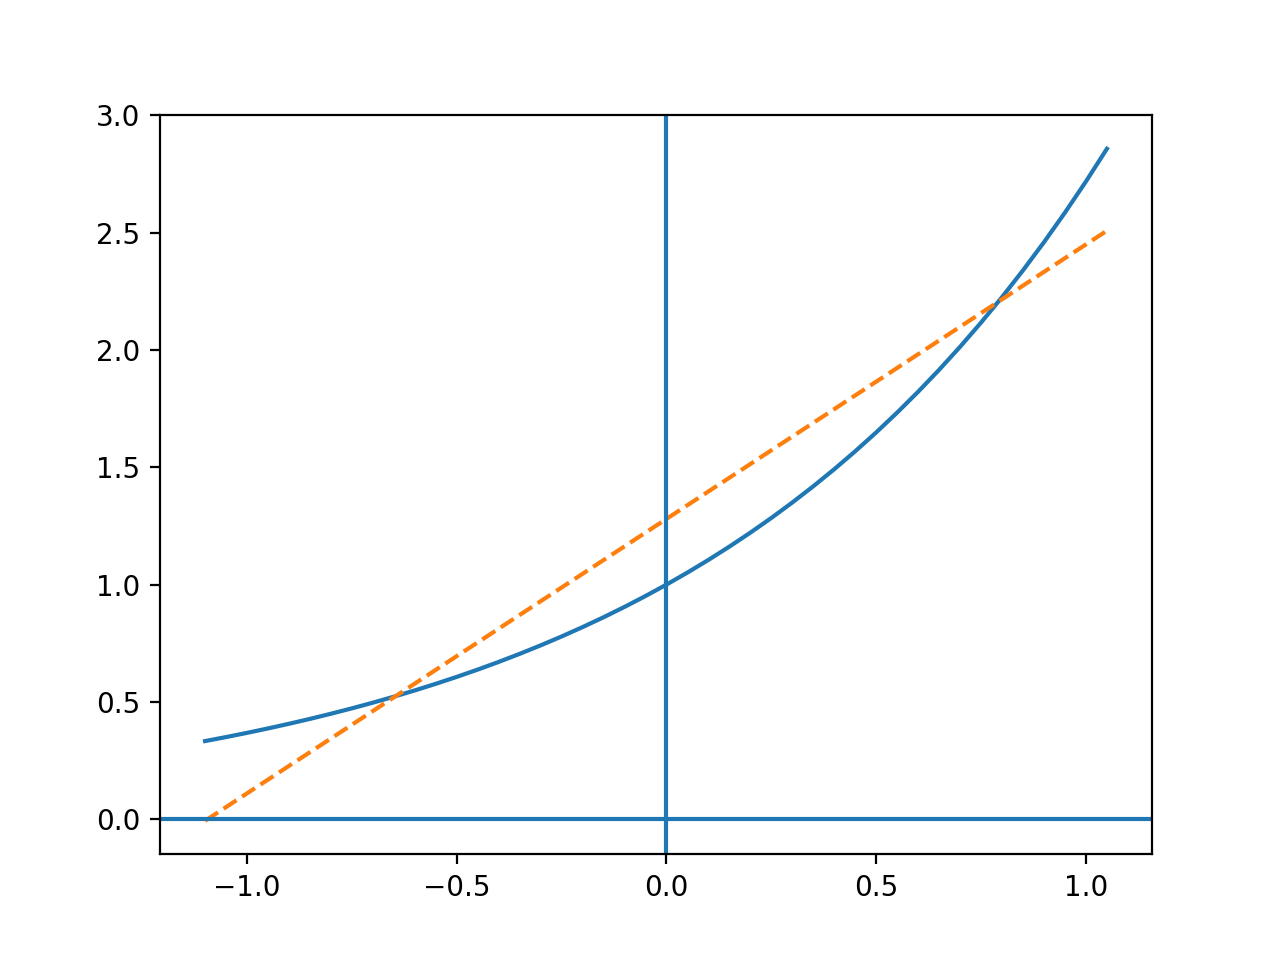
\includegraphics[height=5cm]{figure_1}}
  \end{itemize}
\end{frame}

\begin{frame}
  \frametitle{Fitting the line}
  \begin{itemize}
  \item So we have three points
  \item $x_0 = -1$, $x_1 = ? $ and $x_2 = 1$ 
  \item at which the error is $f(x) = p(x)$
  \item So what  is $x_1$?
    \pause
  \item we can write $p(x) = a + b x$
  \item We can compute the error at the three points:
    \[
      \begin{array}{llll}
        e(x_0) & = f(x_0) - p(x_0) & = f(-1) - p(-1) & = \frac{1}{e} - a + b\\
        e(x_1) & = f(x_1) - p(x_1) &                 & = e^{x_1} - a + b x_1\\
        e(x_2) & = f(x_2) - p(x_2) & = f(1) - p(1)   & = e - a - b\\
      \end{array}
    \]  
  \item Given $e(x_0) = e(x_2)$
    \[
      \begin{array}{ccc}
        \frac{1}{e} - a + b & = & e - a - b\\
        2 b & = & e - \frac{1}{e} \\
        b   & = & 1.1752\\
      \end{array}
    \] The slope is equal to the average change
  \end{itemize}
\end{frame}

\begin{frame}
  \frametitle{Fitting the line (cont)}
  \begin{itemize}
  \item How do we find a? 
  \item The difference (positive / negative) should be symmetric
  \item The error function should at an extrema at $x_0, x_1, x_2$ but with alternate signs
  \item $e(x) = f(x) - p(x) = e^x - a - b x$ so 
  \item $e'(x) = e^x - b$ $\Rightarrow$ $ e^{x_1} -b = 0$
  \item $x_1 = ln ~ b$
  \item $x_1 \approx 0.16144$ \pause
  \item $e(x_1) = -e(x_2)$ $\Rightarrow$ $e^{x_1} - a - b x_1 = -e + a + b$
  \item $a = \frac{e-b x_1}{2} \approx 1.2643$
  \item $p(x) \approx 1.2643 + 1.1752 x$
  \item The maximum error would be $e(x_1) = ||f(x_1) - p(x_1)||_{\infty} \approx 0.2788$    
  \end{itemize}
\end{frame}

\begin{frame}
  \frametitle{Approximation - Discussion}
  \begin{itemize}
  \item Example showed a way to construct a solution.
  \item What if we did not know the appropriate n?
  \item If we make n too small there is a lack of fit
  \item If we make n too large the fit will be poor (too much wiggle)
  \item Could we estimate $d(f, \pi_n)$? 
  \item Maybe not, but a lower bound might be possible    
  \end{itemize}
\end{frame}

\begin{frame}
  \frametitle{Divided Differences}
  \begin{itemize}
  \item Slight detour
  \item Divided differences are frequently used to compute coefficients in interpolation polynomials. 
  \item Recursive formulation. Given a set of data points $(x_0, y_0),\ldots,(x_k,y_k)$
    \[
      [y_v, \ldots, y_{v+j}] = \frac{[y_{v+1}, \ldots, y_{v+j}] - [y_v,\ldots,y_{v+j-1}]}{x_{v+j} - x_v}
    \] and
    \[ [y_v] = y_v \mbox{ ~~~ } v \in \{0, \ldots, k\} \]
  \item The recursive formulation is computationally effective
  \item The first few terms
    \[
      \begin{array}{rcl}
        \mbox{[} y_0 ]           & = & y_0\\ 
        \mbox{[} y_0, y_1 ]      & = & \frac{y_1 - y_0}{x_1 - x_0}\\
        \mbox{[} y_0, y_1, y_2 ] & = & \frac{[ y_1,y_2 ] - [ y_0,y_1 ]}{x_2 - x_0}
                              = \frac{\frac{y_2-y_1}{x_2-x_1} - \frac{y_1-y_0}{x_1-x_0}}{x_2 - x_0}\\
                        & = & \frac{y_2 - y_1}{(x_2-x_1)(x_2-x_0)} - \frac{y_1 - y_0}{(x_1-x_0)(x_2-x_0)}\\
      \end{array}
    \]
  \end{itemize}
\end{frame}

\begin{frame}
  \frametitle{Estimating a lower bound}
  \begin{itemize}
  \item Assume we have a function $f:[a,b] \rightarrow R$
  \item We will use divided differences to compute bounds
  \item Lets assume we have three points $x_0, x_1, x_2$ as p is linear
    \[
      p[x_0, x_1, x_2] = 0
    \] i.e. the gradient does not vary
  \item we can also write
    \[
      f[x_0, x_1, x_2] = \frac{f(x_0)}{(x_0-x_1)(x_0-x_2)}+
      \frac{f(x_1)}{(x_1-x_0)(x_1-x_2)}+
      \frac{f(x_2)}{(x_2-x_0)(x_2-x_1)}
    \] so 
  \end{itemize}
\end{frame}


\begin{frame}
  \frametitle{Estimating lower bound (cont.)}
    \[
      \begin{array}{rcl}
        f[x_0, x_1, x_2] &=&  f[x_0, x_1, x_2] -  p[x_0, x_1, x_2]\\ 
                         &=&  (f-p)[x_0, x_1, x_2]\\ 
                         &=& \frac{f(x_0)-p(x_0)}{(x_0-x_1)(x_0-x_2)}+
                             \frac{f(x_1)-p(x_1)}{(x_1-x_0)(x_1-x_2)}+
                             \frac{f(x_2)-p(x_2)}{(x_2-x_0)(x_2-x_1)}\\
                         &=& \frac{f(x_0)-p(x_0)}{w'(x_0)}+
                             \frac{f(x_1)-p(x_1)}{w'(x_1)}+
                             \frac{f(x_2)-p(x_2)}{w'(x_2)}\\
      \end{array}      
    \] where
    \[
      w'(x) = (x-x_0)(x-x_1)(x-x_2)
    \]
\end{frame}

\begin{frame}
  \frametitle{Estimating lower bound (cont.)}
  \begin{itemize}
  \item We can then estimate a bound
    \[
      | f[x_0,x_1,x_2] | \leq ||f-p||_{\infty}
      \left( \frac{1}{|w'(x_0)|} + \frac{1}{|w'(x_1)|} + \frac{1}{|w'(x_2)|} \right)
    \] or
    \[
      ||f-p||_{\infty} \geq \frac{| f[x_0,x_1,x_2] | }{\frac{1}{|w'(x_0)|} + \frac{1}{|w'(x_1)|} + \frac{1}{|w'(x_2)|}}
    \]
  \item the polynomial on left hand side is arbitrary so $d(f,\pi_n) = min_{p\in \pi_n}||f-p||_{\infty}$
  \item right hand side is purely based on f and three points, so we can estimate the value
  \end{itemize}
\end{frame}

\begin{frame}
  \frametitle{Back to our example}
  \begin{itemize}
  \item Lets use $f(x) = e^x$ in the interval $[-1,1]$. 
  \item Pick say -1, 0, 1 as our points
    \[
      f[x_0,x_1,x_2] = \frac{1}{2} f(-1) - f(0) + \frac{1}{2} f(1)
    \] and
    \[
      \frac{1}{|w'(x_0)|} + \frac{1}{|w'(x_0)|} + \frac{1}{|w'(x_0)|} = \frac{1}{2} + 1 + \frac{1}{2} = 2
    \] thus
    \[
      d(f,\pi_1) \geq \frac{f(-1) - 2 f(0) + f(1)}{4} 
    \]
  \item the bound is then $d(f,\pi_1) = 0.2715$, which is not too far away from 0.2788 that was achieved. 
  \item the lower bounds says that we cannot estimate $e^x$ much
    better than .3 in the interval -1,1 with a linear approximation,
    which is very valuable.
  \end{itemize}
\end{frame}

\section{Chebyshev Approximation}

\begin{frame}
  \frametitle{Chebyshev polynomials}
  \begin{itemize}
  \item Chebyshev polynomials are sequences of polynomials that are defined recursively.
  \item The first kind of a Chebyshev polynomial is denoted $T_N(x)$ and given by
    \[
      T_N(x) = \cos( n \arccos x)
    \]
    looks trigonometric but can be used to general polynomials. I.e
    \[
      \begin{array}{rcl}
        T_0(x)     & = & 1\\
        T_1(x)     & = & x\\
        T_2(x)     & = & 2 x^2 - 1 (\mbox{as } cos(2\theta) = 2cos^2(\theta) -1) \\ 
        T_3(x)     & = & 4 x^3 - 3 x \\
        T_{N+1}(x)  & = & 2 x T_N(x) - T_{N-1}(x), \mbox{ for } n \geq 1\\
      \end{array}
    \]
  \end{itemize}
\end{frame}

\begin{frame}
  \frametitle{Chebyshev Polynomials}
  \begin{itemize}
  \item The polynomials are orthogonal over the interval $[-1,1]$ over a weight of $(1-x^2)^{-1/2}$ so that
    \[
      \int_{-1}^2 \frac{T_i(x) T_j(x)}{\sqrt{1-x^2}} dx = \left\{
        \begin{array}{ll}
          0& i \neq j\\
          \frac{\pi}{2} & j = j \neq 0\\
          \pi & i = j = 0
        \end{array}\right.
    \]
  \end{itemize}
\end{frame}

\begin{frame}
  \frametitle{Chebyshev Polynomials}
  \begin{itemize}
  \item The polynomial $T_N(x)$ has N zeros in the internal $[-1,1]$ at the points $x=\cos(\frac{\pi (k+\frac{1}{2})}{N})$ for $k \in 0, \ldots, N-1$
  \item It is a similar set of extrema at $x = \cos(\frac{\pi k}{N})$
    \centerline{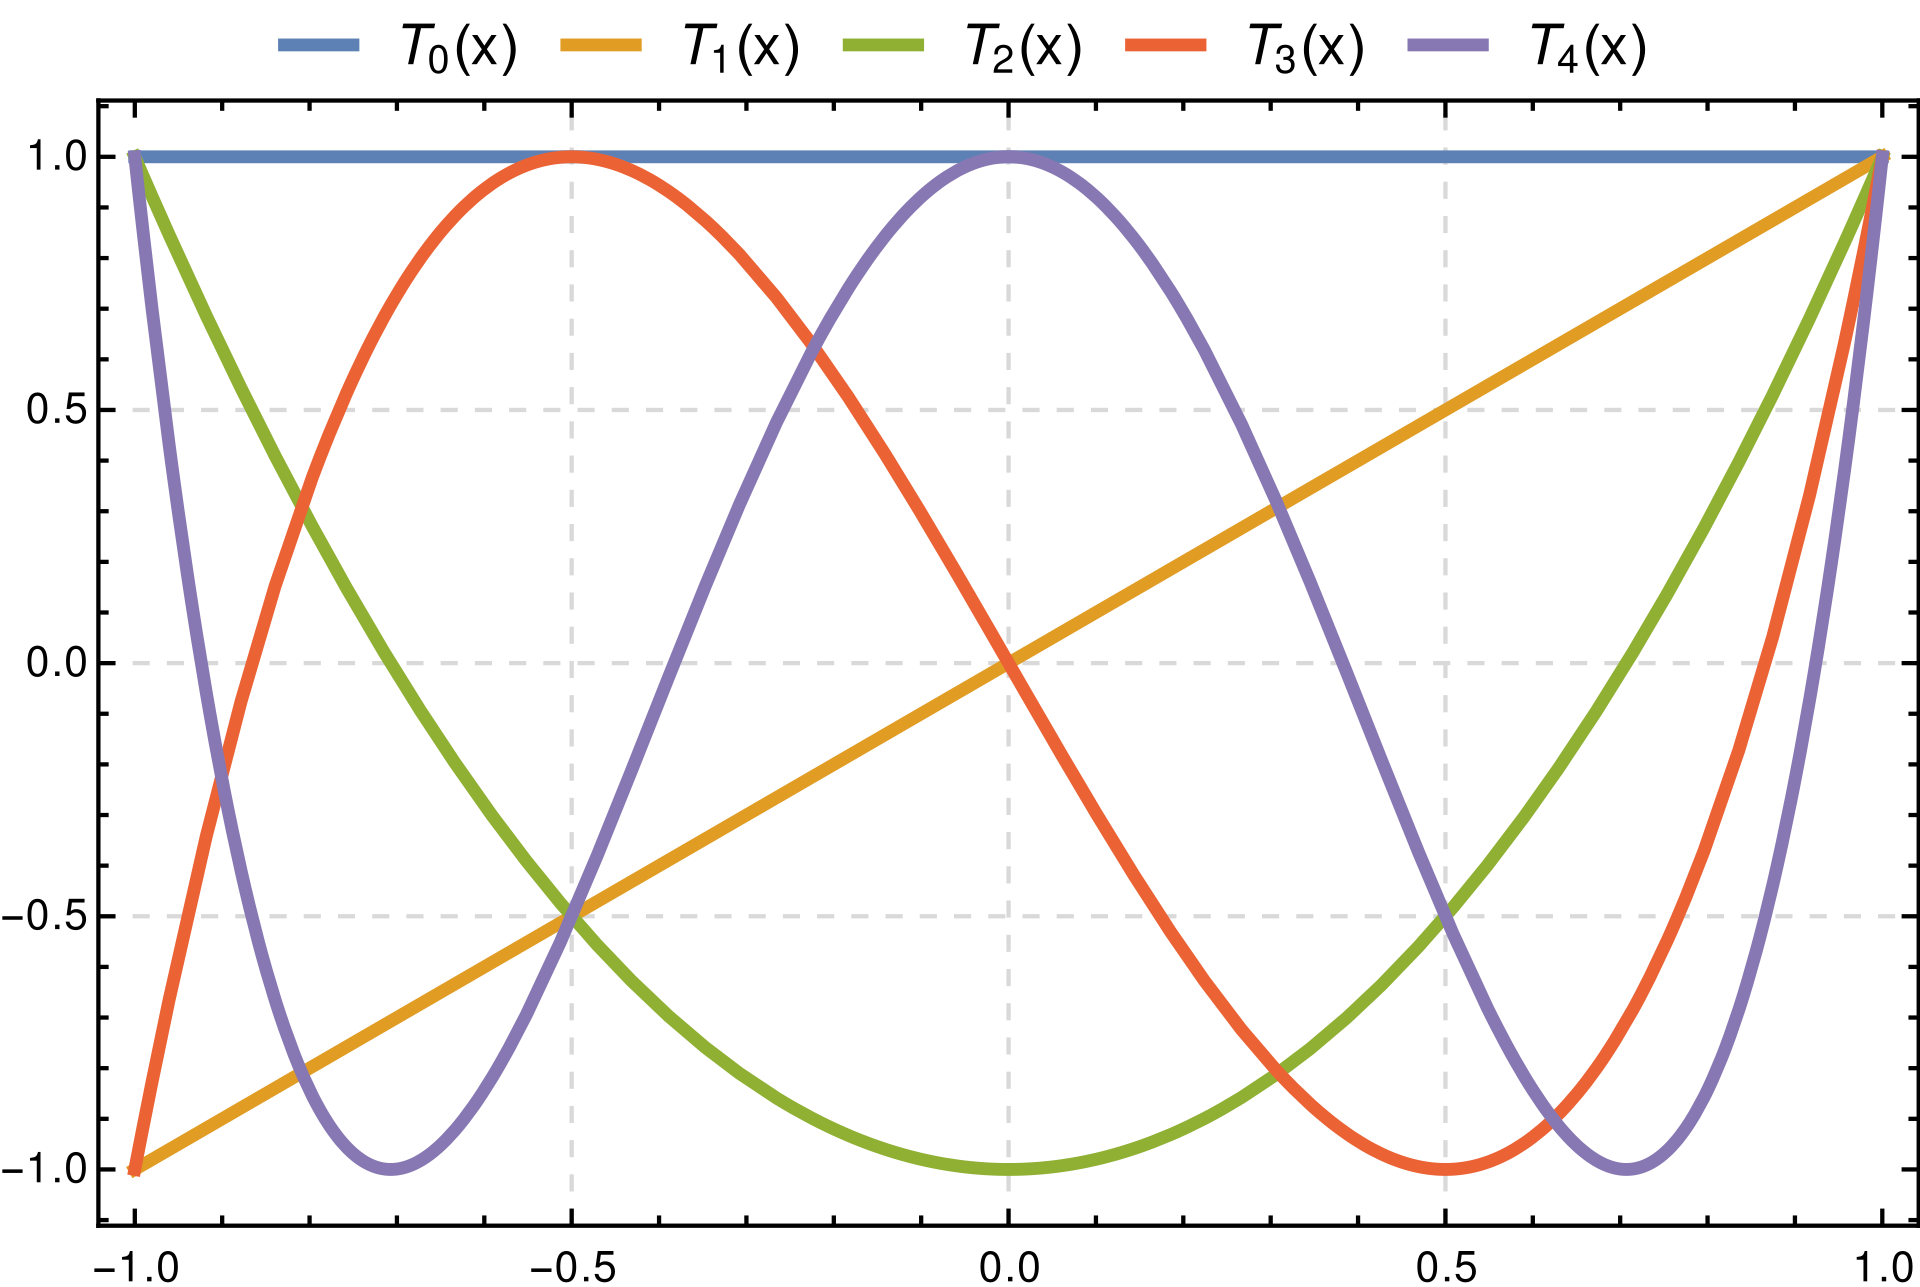
\includegraphics[height=4cm]{Chebyshev}}
  \end{itemize}
\end{frame}

\begin{frame}
  \frametitle{Chebyshev Approximation}
  \begin{itemize}
  \item For periodic functions. f(x), over the interval $[-1,1]$ an N coefficient approximation is
    \[
      \begin{array}{rcl}
      c_j & = & \frac{2}{N} \sum_{k=0}^{N-1} f(x_k) T_J(x_k)\\
          & = & \frac{2}{N} \sum_{k=0}^{N-1} f\left( \cos \frac{\pi (k+\frac{1}{2})}{N} \right) \cos \frac{\pi (k+\frac{1}{2})}{N} \\
      \end{array}
    \]
  \item The approximation is then
    \[
      f(x) \approx p(x) = \left[ \sum_{k=1}^{N-1} c_k T_k(x) \right] - \frac{1}{2} c_0
    \]
  \item which is an exact match in terms of zero crossings
  \item the errors are uniformly distributed over $[-1,1]$     
  \end{itemize}
\end{frame}

\begin{frame}
  \frametitle{Warping coordinated}
  \begin{itemize}
  \item If the domain is different from $[-1,1]$ the variable can be changed from $[a,b]$
    \[
      y = \frac{x -\frac{1}{2} (b-a)}{\frac{1}{2}(b-a)}
    \]
    the approximated can be mapped forward / back as needed
  \end{itemize}
\end{frame}

\begin{frame}
  \frametitle{Example of using Checyshev Points for Control}
  \centerline{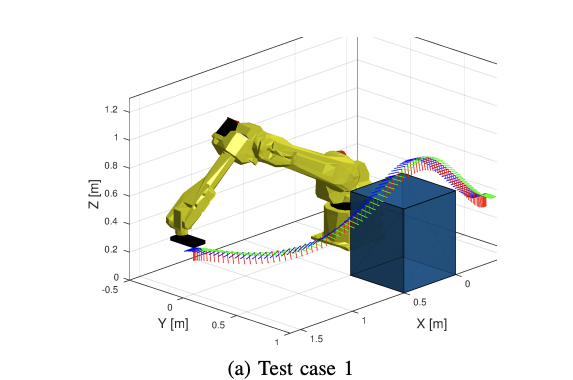
\includegraphics[height=6cm]{Chebyshev-points}}
\end{frame}

\section{Truncated Power Series}

\begin{frame}
  \frametitle{Truncated Power Series}
  \begin{itemize}
  \item The uniform error of the Chebyshev functions/series imples
    that one can use a limited number of terms
  \item Say you have a series
    \[
      f(x) = \frac{1}{2} - \frac{x}{4} + \frac{x^2}{8} - \frac{x^3}{16} + \ldots
    \]
  \item fitting a polynomial function and trying to achieve
    $\epsilon < 10^{-9}$ would require more than 30 terms
  \item If we use a Chebyshev approximation
    \begin{enumerate}
    \item Compute enough terms to have $\epsilon < T$ across series
    \item Change variable to $[-1,1]$
    \item Find Chebyshev series that satisfy error
    \item Truncate series using $c_kT_k(x)$ as an estimated error residential
    \item Convert back to polynomial form
    \item Convert back to original coordinate range
    \end{enumerate}
  \item For the example the reduction is from 30 to 9 terms
  \end{itemize}
\end{frame}

\section{Summary}

\begin{frame}
  \frametitle{Functional approximation and interpolation}
  \begin{itemize}
  \item Frequently using a functional approximation is much more
    effective and it adds semantic information (a class) to the data
    approximation
  \item The are quite a few functional approximaiton forms
  \item Giving a few examples from polynomial, $\pi_n$, form to periodic function
  \item A key consideration is what domain knowledge is available to guide model selection
  \end{itemize}
\end{frame}

\begin{frame}
  \frametitle{Small example}
  \centerline{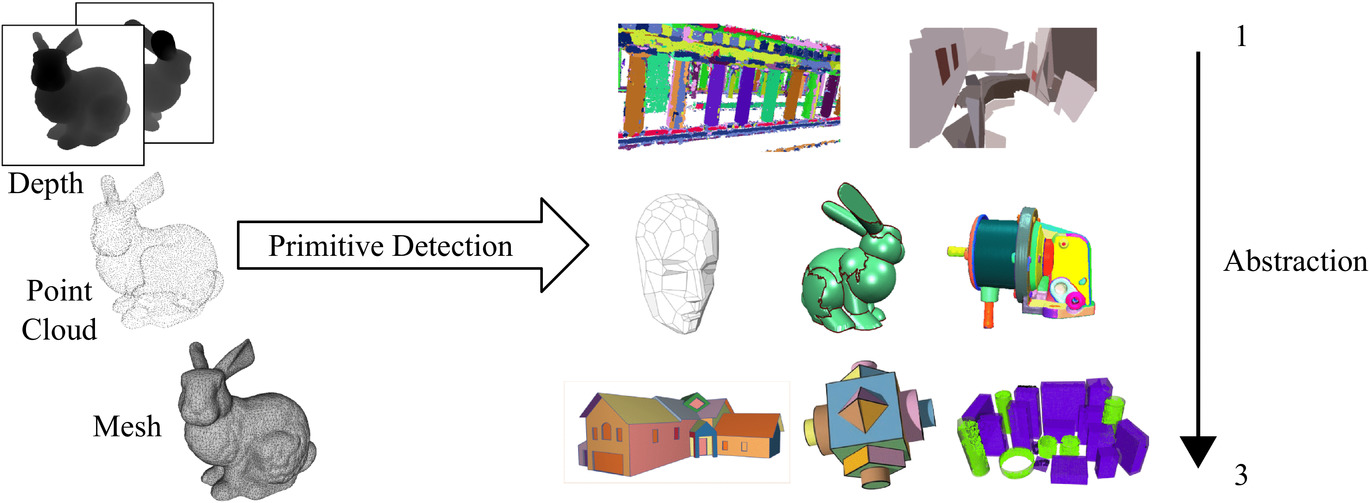
\includegraphics[width=10cm]{primitives}}
\end{frame}

\begin{frame}
  \frametitle{Questions}
  \centerline{\Huge Questions}
\end{frame}

\end{document}

%%% Local Variables:
%%% mode: latex
%%% TeX-master: t
%%% End:
